\subsection{Induction}
\hrulefill

\paragraph*{Definition}
Induction is the process of generating an electromotive force in a closed circuit by changing the magnetic field around the circuit.
It is the basis of many electrical devices, including transformers and generators. Induction is governed by Faraday's Law of Induction,
which states that the induced electromotive force in a circuit is equal to the negative rate of change of the magnetic flux through 
the circuit. This is given by the following equations:

\begin{align*}
    \varepsilon &= -\frac{d\Phi_B}{dt} = -\frac{\Delta \Phi_B}{\Delta t}\\
    \varepsilon &= -N\frac{d\Phi_B}{dt} = -N\frac{\Delta \Phi_B}{\Delta t}\\
    \varepsilon &= \frac{d}{dt}(BA\cos(\theta)) = -BA\sin(\theta)
\end{align*}

Where $\varepsilon$ is the electromotive force in volts, $N$ is the number of turns in the coil, $\Phi_B$ is the magnetic flux in webers,
$B$ is the magnetic field in teslas, $A$ is the area of the coil in square meters, and $\theta$ is the angle between the magnetic field
and the normal to the coil.\\

FORMAT THIS: 
\begin{align*}
    \Phi_B &= \int \vec{B} \cdot d\vec{A} = BA = B\ell w\\
    \varepsilon &= \frac{B^2\ell^2v}{R}
\end{align*}

\begin{center}
    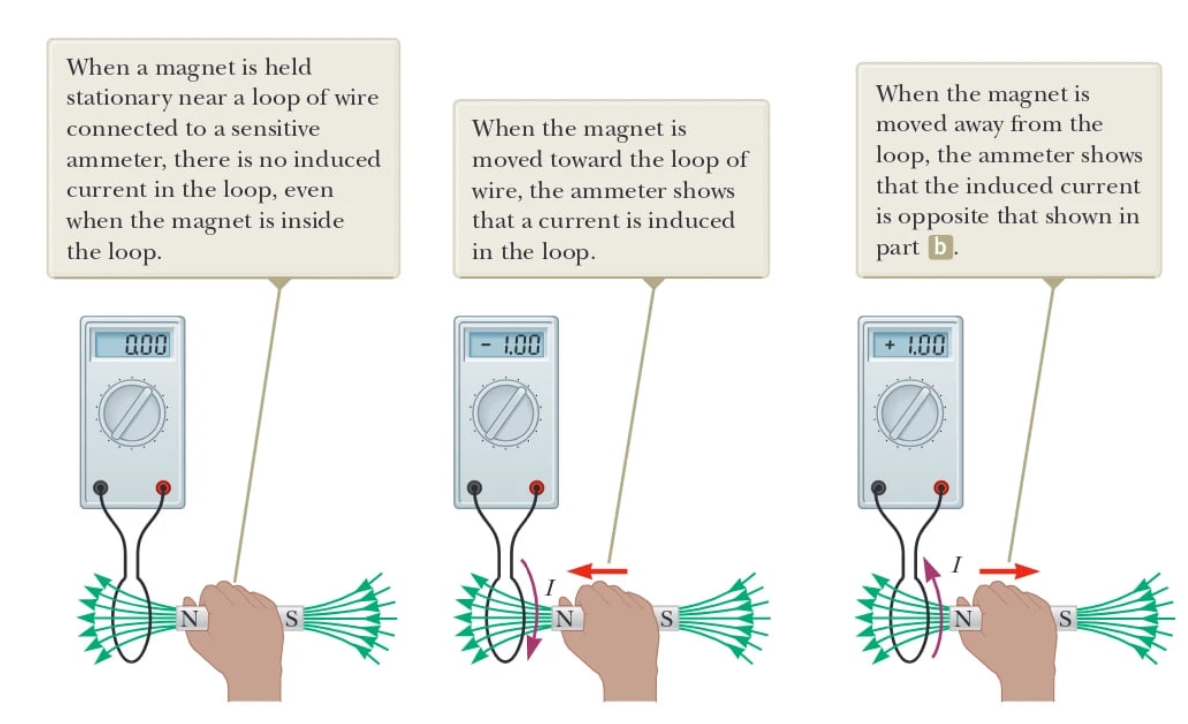
\includegraphics[scale=0.5]{induction.png}
\end{center}

\paragraph*{Lenz's Law}
Lenz's Law states that the direction of the induced current in a circuit is such that it opposes the change in magnetic flux that caused it. 
Practically, this means that when the magnetic flux increases, an opposing magnetic field is generated to counteract the increase. 
Conversely, if the magnetic flux decreases, the generated magnetic field will be in the same direction as the original field, opposing the 
decrease. The direction of this opposing field determines the direction of the induced current.

\begin{center}
    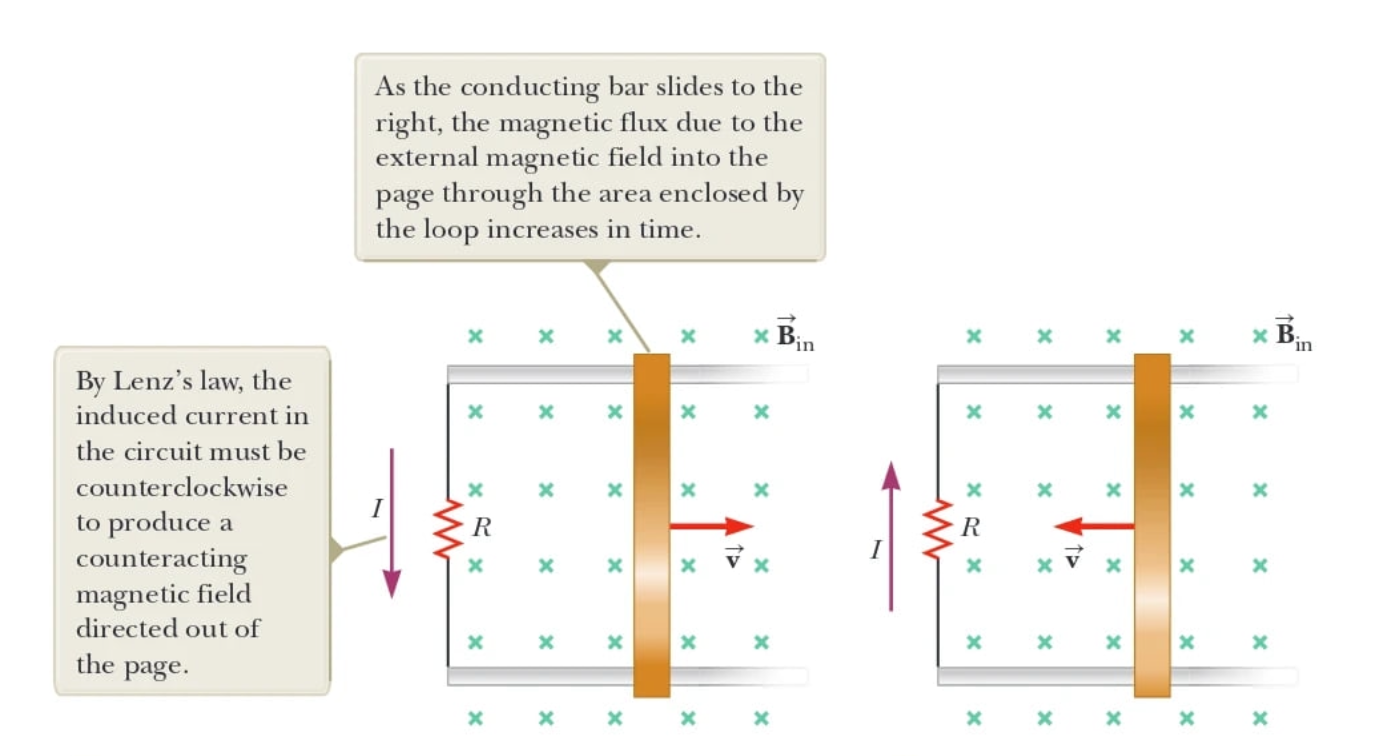
\includegraphics[scale=0.5]{lenz_law.png}
\end{center}


\begin{wrapfigure}[5]{r}{0.3\textwidth}
    \centering
    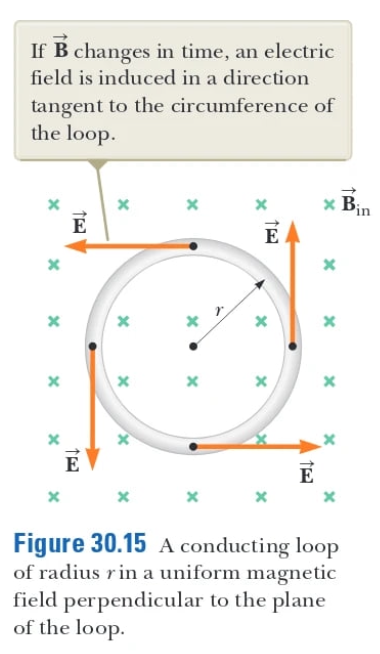
\includegraphics[scale=.5]{faraday.png}
\end{wrapfigure}

\paragraph*{General Form of Faraday's Law}

\begin{align*}
    \oint \vec{E} \cdot d\vec{\ell} &= -\frac{d\Phi_B}{dt}
\end{align*}



Which allows us to find the Electric Field generated by a changing magnetic field.

\begin{align*}
    E &= -\frac{r}{2}(\frac{dB}{dt})
\end{align*}

Where $\vec{E}$ is the electric field in volts per meter, $d\vec{\ell}$ is an infinitesimal segment of the circuit in meters, $\Phi_B$ is the
magnetic flux in webers, $r$ is the distance from the wire in meters, and $\frac{dB}{dt}$ is the rate of change of the magnetic field in 
teslas per second.\\


\paragraph*{Self-Inductance}
Self-inductance is the property of a circuit that causes it to generate an electromotive force in response to a change in current.
It is measured in henries $[H] = [V\cdot \frac{s}{A}]$. The electromotive force generated by self-inductance is given by the following equation.

\begin{align*}
    \varepsilon &= -L\frac{dI}{dt}
    L &= \frac{\varepsilon_L}{dI/dt} = \frac{N\Phi_B}{I}
\end{align*}

Where $\varepsilon$ is the electromotive force in volts, $L$ is the self-inductance in henries, $I$ is the current in amperes, $N$ is the 
number of turns in the coil, and $\Phi_B$ is the magnetic flux in webers.\\

\subsubsection*{RL Circuits}
\paragraph*{Definition}
An RL circuit is a circuit that contains a resistor and an inductor. When a current is passed through the circuit, the inductor generates
an electromotive force that opposes the change in current. This causes the current to increase more slowly than it would in a circuit with
only a resistor. The current in an RL circuit is given by the following equation.

\begin{align*}
    I(t) &= \frac{\varepsilon}{R}(1 - e^{-t/\tau})
    \tau &= \frac{L}{R}
    I_{max} &= \frac{\varepsilon}{R} 
\end{align*}

Where $I(t)$ is the current in amperes, $\varepsilon$ is the electromotive force in volts, $R$ is the resistance in ohms, $t$ is the time in seconds,
$\tau$ is the time constant in seconds, $L$ is the inductance in henries, and $I_{max}$ is the maximum current in amperes.\\

\paragraph*{Energy in a Magnetic Field}
The energy stored in a magnetic field is given by the following equation.

\begin{align*}
    U_B &= \frac{1}{2}LI^2
\end{align*}

Where $U_B$ is the energy stored in the magnetic field in joules, $L$ is the inductance in henries, and $I$ is the current in amperes.\\

\paragraph*{Mutual Inductance}
Mutual inductance is the property of a circuit that causes it to generate an electromotive force in response to a change in current in a
neighboring circuit. It is measured in henries. 

\begin{align*}
    M_{12} &= \frac{N_2\Phi_12}{I_1}\\
    M_{21} &= \frac{N_1\Phi_21}{I_2}\\
    \varepsilon_1 &= -M_{21}\frac{dI_2}{dt}\\
    \varepsilon_2 &= -M_{12} \frac{dI_1}{dt}
\end{align*}